\section{实验1:个性化广告生成者感知}
在人工智能逐步渗透内容创作的背景下,受众如何感知AI生成的信息,尤其是个性化广告,仍然是一个尚未充分探索的重要议题。尽管AI生成文本在某些特征上可能与人类文本存在差异,但受众是否能够准确区分AI生成的内容,以及他们对AI作为信息源的感知如何影响个性化广告的接受度,仍值得进一步研究。\citet{bai2023artificial}的研究表明,相较于人类撰写的文本,AI 生成的信息通常被认为更客观、更理性,但较缺乏独特性和叙事性。然而,在信息源不明确的情况下,人们在阅读 AI 生成的信息时,往往不会直接意识到其来源。即使受试者所阅读的信息由AI生成,大多数参与者仍认为这些内容是由人类撰写的。在 AI 生成文本的条件下,94.4\%的参与者认为文本是人类创作的,而在人类文本条件下,该比例为94.7\%。这一发现表明,在某些文本类型下,AI 生成的信息在受众看来与人类创作的文本并无显著差异,受众也并不容易察觉信息的真实来源。

基于此,实验1旨在考察受众在阅读个性化广告时,对广告生成者(AI vs.人类专家)的感知。具体而言,我们关注以下问题:(1)参与者是否能够准确区分 AI 生成的个性化广告与人类专家创作的广告?(2)哪些文本特征可能影响受众对广告信息源的判断?通过探讨参与者的感知偏差,本实验将为后续研究信息来源对个性化广告说服效果的影响提供基础性证据。

\subsection{方法}

本实验采用 \textbf{2(信息创作者:AI/人类专家)}的被试间设计。AI条件选取当前表现最优的模型GPT-4,人类专家以心理学专业研究生作为代表。广告通过针对五种不同人格水平(外倾性、开放性、尽责性、宜人性、神经质)的高水平特质进行个性化设计,即分别为高外倾、高开放、高尽责、高宜人和高神经质的消费者设计了广告内容。每位被试被随机分配到一类信息创作者的广告条件,并从每个人格水平对应的 3 则广告中随机选择 1 则进行呈现。被试依次观看五则广告(对应五种人格水平),广告呈现顺序随机,且需对每则广告进行评价。

\subsubsection{被试}

通过见数平台发布实验,366名参与者自愿参加这项研究。28名参与者由于注意检查测试未通过被剔除,剩余\textbf{322}名有效被试(年龄范围= 18-58岁;\textit{M}=29.43岁;\textit{SD}=7.36;女性203名)。参与任务的每名参与者获得5元人民币作为报酬。其中注意力检测题为一道见数平台自带的题目:“今天天气不错,请选2”,若未选2,则被判定为注意力检测题未通过。

\subsubsection{实验材料}
针对2(信息创作者:AI/人类专家)*5(广告人格:外倾性/开放性/尽责性/宜人性/神经质)共10个条件生成广告材料。AI条件选取当前表现最优的模型GPT,人类专家以心理学专业研究生作为代表。根据前人文献选择中性的产品手机,广告描述避免具体品牌名以排除品牌的影响。提供给GPT和人类专家的指导语是相同的,包括对目标消费者特点的描述(个性化,具体的人格描述参考人格特质量表中的描述)以及广告基本特征的描述。每类信息创作者(AI/人类专家)针对每种人格水平生成3-5则广告。

\subsubsection{问卷测量}
本实验采用单项选择题评估参与者对个性化广告生成者的感知。具体而言,参与者在阅读每则广告后,回答“你认为这则广告的撰写者最可能是?”。选项包括:普通人/广告专家/人工智能。

\subsubsection{文本分析}
为进一步探讨广告文本的哪些特征可能影响受试者对其来源的推测,本研究采用 LIWC(Linguistic Inquiry and Word Count) 进行文本分析(详细介绍见\ref{LIWC})。鉴于本实验的核心关注点是广告来源的归因差异,因此文本分析主要聚焦于词法和句法相关的特征,以识别可能导致受试者推测广告来源为普通人、广告专家或人工智能的语言模式。具体而言,本研究主要关注 词长(Sixltr)、助词(Particle)、分析思维(Analytic)、句子长度(Words per sentence) 等句法结构特征,以及 代词使用(Pronoun)、功能词(Function words)、标点符号(Punctuation) 等可能影响文本可读性和风格的语言模式。


\subsection{结果}

为检验广告创作者(GPT-4 vs. 人类专家)是否影响受试者对广告来源的归因,本研究采用 \textbf{卡方检验)} 进行分析。结果表明(如图\ref{fig:Study4-exp1-perception}),广告创作者与参与者对广告来源的感知之间存在显著关联,$\chi^2(2) = 18.50, \textit{p} < .001$。具体而言,GPT-4 生成的广告更倾向于被归因为 AI 生成,而人类专家撰写的广告更可能被受试者认为是普通人创作的。这一发现表明,即便在广告创作者未知的情况下,参与者仍然能够在一定程度上区分AI生成和人类创作的广告,反映出 AI 生成广告在语言特征或表达方式上的潜在区别。

\begin{figure}[H]
    \centering
    \subfloat[GPT 创作者]{
        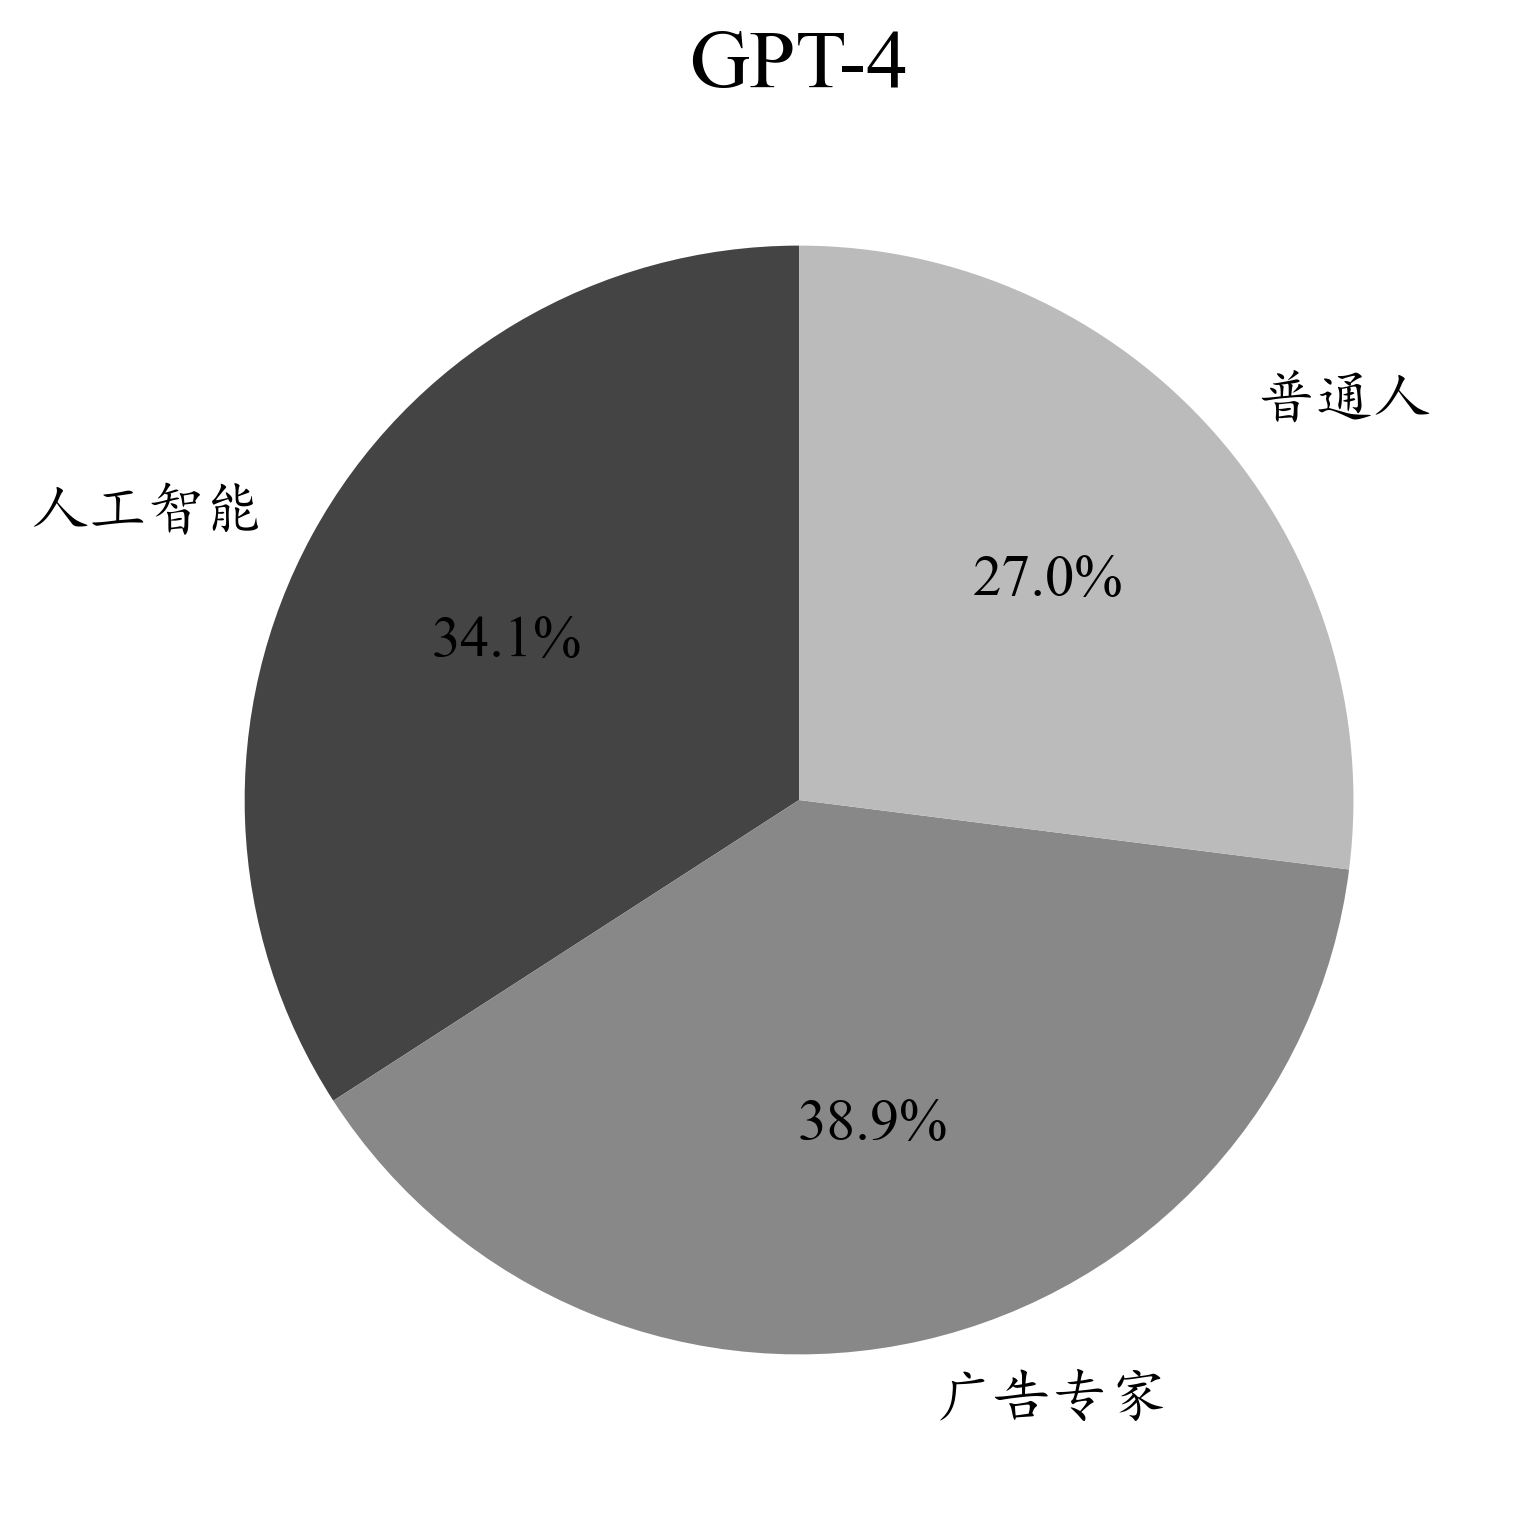
\includegraphics[width=0.4\linewidth]{Image/Study4-exp1-GPT创作者.png}
    }\hspace{2em} % 控制两张图片之间的水平间距
    \subfloat[人类专家创作者]{
        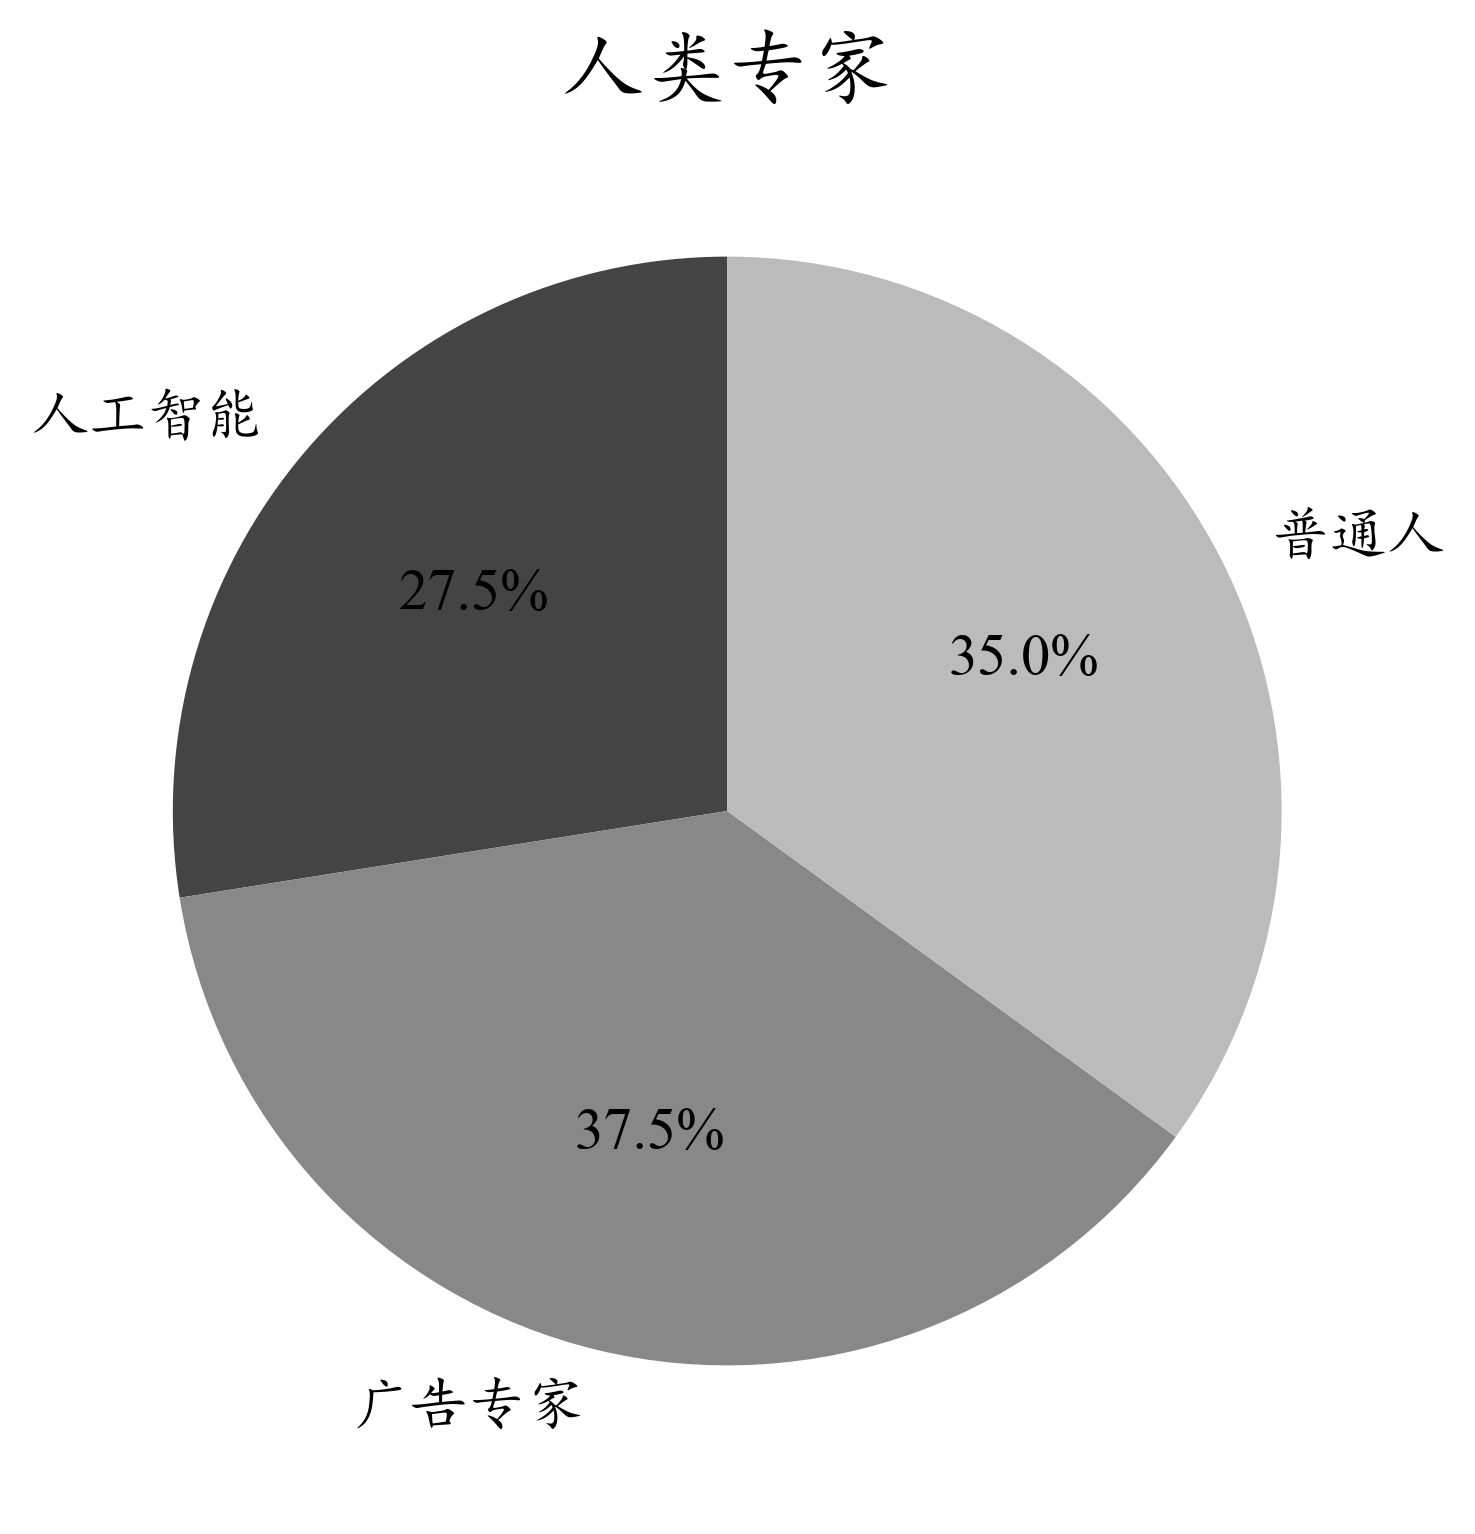
\includegraphics[width=0.4\linewidth]{Image/Study4-exp1-人类专家创作者.png}
    }
    \caption{\label{fig:Study4-exp1-perception} GPT与人类专家实验材料的创作者感知}
\end{figure}

为进一步探讨广告文本的语言特征如何影响受试者对广告来源的推测,本研究基于 LIWC 词法和句法特征进行了单因素方差分析(ANOVA),比较不同广告创作者(AI 生成 vs. 广告专家撰写 vs. 普通人撰写)之间的语言差异。分析结果表明(如表\ref{tab:Study4-substudy1-linguistic_features},不同来源的广告在词汇复杂度、句法结构、指代用法、否定表达、语气表达及冠词使用等方面存在显著差异。

在词汇复杂度方面,AI 生成的广告文本使用了更多的长单词(Sixltr,即包含六个及以上字母的词),其比例最高(0.152),其次是广告专家(0.149),而普通人撰写的广告使用长单词的比例最低(0.033)。这一结果表明,AI 生成的广告语言可能更加正式和专业,而人类撰写的广告更偏向于口语化表达。此外,在句法复杂度方面,AI 生成的广告在句均词数(WPS)上表现出一定优势(22.98),与广告专家(23.31)相近,但均显著高于普通人撰写的广告(22.26)。这表明 AI 生成的广告倾向于使用更长、更复杂的句子,使文本显得更加流畅和结构化,但同时可能降低其口语化程度。

在代词使用方面,AI 生成的广告文本更少使用不定代词(ipron,如“它”“任何”“每个人”),其使用频率最低(1.14),广告专家次之(1.29),而普通人撰写的广告使用最多(1.57)。这一结果可能表明,AI 在生成文本时更注重信息的清晰性,减少了含糊的指代,而人类撰写的广告则更倾向于随意使用不定代词,使文本更具互动感和自然性。此外,在否定表达和比较表达方面,普通人撰写的广告更倾向于使用否定词(negate,如“不会”“没有”),其使用比例最高(1.12),而广告专家使用最少(0.90),AI 生成的广告位于中间(1.21)。相反,AI 生成的广告在比较级(compare,如“更好”“最佳”)的使用频率最高(3.60),其次是广告专家(3.25),而普通人使用最少(3.06)。这一结果表明,AI 生成的广告更倾向于使用比较表达,可能是为了增强广告的说服力,而人类广告撰写者在表达时更直接、更少使用否定表达。

在语气表达方面,AI 生成的广告更倾向于使用推测性语言(discrep,如“应该”“可能”“可以”),其使用比例最高(2.09),普通人次之(1.82),广告专家最低(1.69)。这表明 AI 生成的广告更容易使用可能性或假设性表达,如“你可以实现……”或“这可能会提升你的体验”,而人类广告撰写者更倾向于使用更加确定性的语言,使广告更具信任感。这一结果说明,AI 生成的广告更偏向于正式表达,而人类撰写的广告更倾向于口语化.

最后,在句子结构方面,AI 生成的广告比普通人撰写的广告更频繁地使用前置词(prepend,如“在……之后”“在……之前”),AI 和广告专家的使用比例相同(1.49),均显著高于普通人(1.18)。这表明 AI 生成的广告文本可能更倾向于使用结构更复杂的句式,而人类撰写的广告更偏向简洁直白的表达方式。

综上所述,AI 生成的广告在多个语言维度上表现出与人类撰写广告的显著差异,尤其是在词汇复杂度、句法复杂度、比较表达、推测性语言和句子结构方面更具特点。这些语言特征可能影响受试者对广告来源的判断,使他们更容易将 AI 生成的广告归因于人工智能,而将人类撰写的广告视为人类专家/普通人创作的内容。


\begin{table}[htbp]
    \centering
    \caption{\label{tab:Study4-substudy1-linguistic_features} 语言特征对比}
    {\tablesongti % 整个表格环境应用宋体六号字体
    \renewcommand{\arraystretch}{1.5} % 调整行距
    \begin{tabular}{l c c c c} % 使用 l 让第一列自动调整
        \toprule
        \textbf{语言特征} & \textbf{\( p \) 值}& \textbf{人工智能} & \textbf{广告专家} & \textbf{普通人} \\
        \midrule
        Sixltr & 0.0004 & 0.1523 & 0.1490 & 0.0329 \\
        WPS & 0.0135 & 22.9795 & 23.3107 & 22.2591 \\
        ipron & 0.0079 & 1.1374 & 1.2979 & 1.5702 \\
        negate & 0.0349 & 1.2136 & 0.9048 & 1.1243 \\
        compare & 0.0288 & 3.6045 & 3.2537 & 3.0647 \\
        discrep & 0.0371 & 2.0909 & 1.6954 & 1.8252 \\
        specart & 0.0421 & 2.2395 & 2.2705 & 1.8440 \\
        prepend & 0.0126 & 1.4974 & 1.4973 & 1.1778 \\
        \bottomrule
    \end{tabular}
    }
\end{table}




